\subsection*{Problemformulering}
\addcontentsline{toc}{subsection}{Problemformulering}
Det eksisterende system ufleksibelt, understøtter ikke domæneregler og har meget
lav fejltolerance. Dette påvirker klinikerne og i sidste ende patienterne - da
meget tid går tabt på det eksisterende system og undersøgelser ikke bliver
udført som planlagt.\\
\indent Vi ser en mulighed for at skabe et langt sikrere og mere fleksibelt
system, hvor rekvisitioner og brugere kan spores gennem hele systemet, hvorved
risikoen for potentielt fatale fejl minimeres.\\
\indent \emph{Økonomi.} Aktuelt arbejder 3 sekretærer helt eller delvist med
håndtering af henvisninger. En stor del af arbejdsbyrden vil kunne
reduceres/elimineres og ledende sekretær skønner at der kunne frigøres minimum
én fuldtids sekretær ved en smidigere arbejdsgang. Hertil kommer tabt indtjening
som følge af aflyste/glemte undersøgelser.\\
\subsubsection*{Direkte Interessenter}
\addcontentsline{toc}{subsubsection}{Direkte Interessenter}
\begin{enumerate}
  \item Klinikere - Bestiller undersøgelser
  \item Røntgenlæger - Visiterer undersøgelser og udfører lægeundersøgelser
  \item Radiografer - Visiterer undersøgelser og udfører øvrige
  \item Sekretærer - Booker undersøgelserne
\end{enumerate}

\subsubsection*{Indirekte Interessenter}
\addcontentsline{toc}{subsubsection}{Indirekte Interessenter}
\begin{enumerate}
  \item Ledelse - Økonomiske interesser
  \item Patienter - Interesseret i at visitationen
\end{enumerate}
\subsection*{Domæne dataindsamling (Christian, Magnus)}
\addcontentsline{toc}{subsection}{Domæne dataindsamling}
For at samle mest mulig data om domænet overvejede vi de mulige måder at
indsamle data. Da der er begrænset med tid i sundhedsvæsenet, prioriterede vi
dataindsamlingsmetoder, der belastede afdelingen mindst muligt og udviklede
vores modeller/prototyper mest muligt, før vi præsenterede dem for brugerne.\\
\indent Initielt mødtes vi med en læge fra afdelingen, der gav os en
baggrundsorientering om hvordan systemet fungerer i praksis. Vi sørgede herefter
for at indsamle alle relevante dokumenter og analyserede disse (se
\hyperref[Bilag5]{bilag 5 - 9}). Vi valgte ud fra disse at lave en prototype,
før vi interviewede interessenterne for at opnå maksimalt udbytte af
interviews'ne. Da der er tale om følsomme data - patientoplysninger mm. - var
det begrænset hvad der kunne lade sig gøre mht. observationer i praksis - vi fik
lov til at se programmerne i praksis, men fik ikke lov til at tage billeder. Vi
overvejede desuden:\\
\begin{enumerate}
  \item \emph{Spørgeskemaundersøgelse} -Det var ikke praktisk ladesiggørligt at
  bruge spørgeskemaundersøgelser, da det var for tidskrævende for
  interessenterne.
  \item \emph{Workshops} - Igen for tidskrævende for vores interessenter, dog
  ville de personer vi interviewede gerne afprøve vores 2. prototype via et
  link, hvorfor vi satte en cloudløsning op til testbrug:
  (\url{http://rtgrek-area51.rhcloud.com/})
  \item \emph{Rige billeder} - Vi illustrerede arbejdsgangen med et rigt billede
  som vi verificerede med brugerne, se \hyperref[Rigt_billede]{figur \ref*{Rigt_billede}}.
  \item \emph{Forbilleder} - Vi havde ikke mulighed for at se
  alternative/sammenlignelige systemer i drift. Vi har kendskab til løsninger,
  men ikke adgang til dem.
  \item \emph{Use cases} - Vi gennemgik de udviklede use cases med
  interessenterne for at sikre os at vi havde forstået problemdomænet rigtigt.
\end{enumerate}
\subsubsection*{Prototyping (Christian, Morten)}
\addcontentsline{toc}{subsubsection}{Prototyping}
Ud fra vores baggrundsforståelse af emnet udviklede vi en prototype på en
røntgenrekvisition, som vi vil præsentere for vores interessenter, for at
afprøve om vi havde forstået domænet rigtigt (se \hyperref[Bilag10]{bilag
10} eller
\href{https://docs.google.com/forms/d/1mb5n0rR4vUuns_TXM7ai3vY1BZxPrvxd8P4NFjs5igw/viewform}{online}).
\indent Udover prototypen på rekvisitionen, har vi også lavet en prototype på
selve visitationen af rekvisitionerne. Denne blev udviklet i Excel VBA, og
skulle blot illustrere for intressenter, hvordan vi forestiller os at
brugerinterfacet kunne se ud (se \hyperref[Bilag11]{bilag 11}).
\subsubsection*{Interviews med interessenter (Christian)}
\addcontentsline{toc}{subsubsection}{Interviews med interessenter}
I første omgang lykkedes det os at få kontakt til og interviewe tre direkte
interessenter og desuden en indirekte interessent. Grundet travlhed på
afdelingen, måtte vi begrænse os til 20 minutter med hver. Vi anvendte et antal
standardiserede spørgsmål for at afdække relevante
problemstillinger\cite{designing} (se eksempel \hyperref[Bilag12]{bilag 12}). Af
pladshensyn er interview beskrivelserne i \hyperref[Bilag13]{bilag 13}.
\indent Ud fra vores interviews tilpassede vi vores krav til vores system. Det
viste sig at det største problem var tabet af rekvisitioner og en tung
arbejdsgang. Derfor valgte vi at holde fokus på at få en velfungerende
rekvisitionsarbejdsgang. Vores visitationsprototype viste sig at være meget tæt
på ønsket - med enkelte forslag til forbedringer. Rekvisitionsprototypen
afspejlede de reelle papirrekvisitioner og viste sig - i lighed med
papirudgaverne at være noget uoverskuelig. Rekvirenten så gerne at antallet af
sider der skulle udfyldes reduceredes. Vi blev desuden også opmærksom på en del
redundant data, der blev gentaget på de forskellige kontrolskemaer.
\subsection*{Aktørbeskrivelse (Rúni, Magnus)}
\addcontentsline{toc}{subsection}{Aktørbeskrivelse}
Systemet bruges af fire aktører: Klinikere (rekvirent), sekretær (booking),
røntgenlæge (visitator) og administrator. Alle fire aktører har som udgangspunkt
forskellige rettigheder, dog er systemet designet til at en bruger senere kan få
flere rettigheder hvis det bliver nødvendigt.
\begin{itemize}
  \item Administrator har lov til at oprette brugere og bestemme hvilke
  rettigheder de har, han kan ikke slette brugere, men kun gøre dem inaktive.
  Administrator skal ikke have lov til at benytte andre brugeres funktionalitet,
  hvilket gør systemet til et tillidssystem, da administrator ellers nemt kan få
  de rettigheder han vil.
  \item Rekvirenten har mulighed for at udfylde en rekvisition og de tilhørende
  kontrolskemaer. Rekvirenten kan søge på alle rekvisitioner, og hvis de
  afventer visitation eller er blevet godkendt, men ikke bookede, har han
  mulighed for at annullere rekvisitionen, uanset om han er registreret som
  rekvirent på rekvisitionen eller ej.
  \item Visitator kan se alle rekvisitoner og søge i dem, han kan visitere dem,
  skrive kommentare til sin visitation og afvise ikke fyldestgørende rekvisitioner.
  \item Sekretæren kan se alle rekvisitoner og søge i dem, han kan booke
  rekvisitioner eller sende dem til visitation hvis det er nødvendigt.
\end{itemize}
De tilladte overlap mellem brugerroller kan ses i \hyperref[Bilag14]{bilag 14}
\subsection*{Use Cases (Morten, Martin)}
\addcontentsline{toc}{subsection}{Use Cases}
I figur 3 ses en model af de involverede use cases, som vi ville arbejde med. I
forhold til den oprindelige arbejdsgang eliminerede vi en use case, hvor
sekretæren scanner rekvisition.\\
\indent Pre-conditions for alle use cases er at bruger er logget ind.
\FloatBarrier
\begin{figure}[h]
\centering
\makebox[\textwidth]{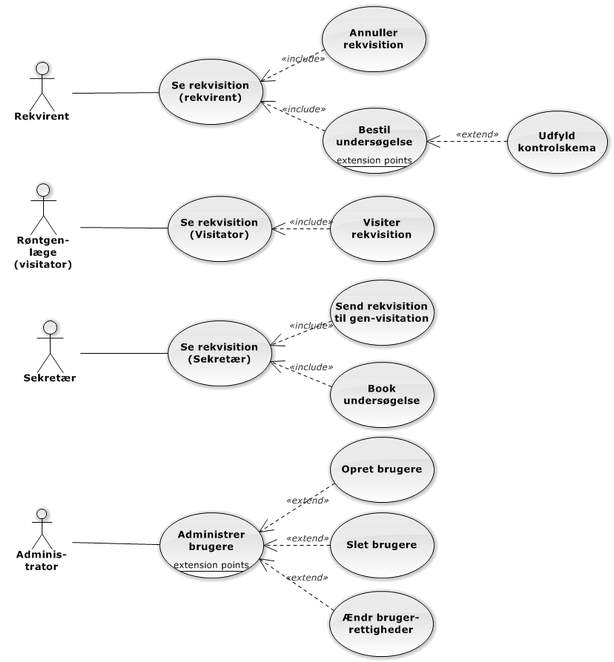
\includegraphics[width=\textwidth]{Usecase_Diagram}}
\caption{\emph{Use case diagram}: Se i øvrigt bilag 15 for tidligere version.
\label{use_case_diagram}}
\end{figure}
\FloatBarrier
\subsection*{Use case beskrivelse (fully dressed): Bestil
undersøgelse\cite{cockburn} (Martin, Morten)}
\addcontentsline{toc}{subsection}{Use case beskrivelse}
\textbf{Primær aktør:} Læge(Rekvirent)\\
\textbf{Mål:} Få en tid til en undersøgelse af en patient.\\
\textbf{Scope:} Rekvisitionssystem til Hillerød hospital.\\
\textbf{Stakeholders and interests:}
\begin{itemize}
  \item Rekvirenter: Vil have en nem, hurtig og sikker måde at sende
  rekvisitioner.
  \item Patienter: Vil komme hurtigt til undersøgelse, og være sikre på at deres
  rekvisition ikke går tabt i systemet samt minimum risiko for fejl i rekvisitionen.
  \item Visitatorer(radiolog): Vil have at data er indtastet korrekt, og er nemt
  at søge i.
  \item Radiografer: Vil have data korrekt indtastet, så de kan lave den rigtige
  undersøgelse.
  \item Sekretærer: Vil gerne have at data er indtastet korrekt i rekvisitionen.
  \item Administratorer: Vil have et sikkert og velfungerende system.
  \item Hillerød hospital: Vil skære unødvendige arbejdstimer for at spare
  penge, og have et sikkert system, da mange rekvisitioner i øjeblikket går tabt
  pga. dårligt system.
  \item Skatteyderen: Vil have deres skattepenge brugt optimalt.
\end{itemize}
\textbf{Precondition:} Alle aktører er logget ind.\\
\textbf{Minimum garanti:} Rekvisition bliver afsendt.\\
\textbf{Success garanti:} Rekvisitionsoplysninger er korrekt indtastet og
afsendt, visitatoren har godkendt rekvisitionen, sekretæren har booket en tid,
data er gemt i systemet.\\
\textbf{Main success scenario:}
\begin{enumerate}
  \item Rekvirent logger ind
  \item Opretter en rekvisition
  \item Indtaster oplysninger i rekvisitionen, og vælger den rigtige modalitet
  \item Udfylder evt. kontrolskema og trykker submit
  \item En visitator logger ind
  \item Vælger den pågældende rekvisition
  \item Godkender undersøgelsen
  \item Sekretæren logger ind
  \item Vælger den pågældende godkendte rekvisition
  \item Booker en undersøgelse til patienten.
\end{enumerate}
\textbf{Extensions:}
\begin{description}
\item[*a)]Hvis systemet går ned, genstartes webserveren af IT-afdelingen.
\item[2-4a)]Hvis brugeren er i gang med at indtaste en rekvisition, og vil
fortryde oprettelsen, kan dette ske ved enten at lukke rekvisitionen på det
store X eller trykke på ESC på tastaturet.
\item[6-7a)]Hvis to visitatorer åbner samme rekvisition, kan den kun godkendes
eller afvises én gang.
\begin{enumerate}
  \item Den visitator der godkender/afviser sidst, får at vide at rekvisitionen
  allerede er behandlet.
  \item Rekvisitionens status ændres ikke.
\end{enumerate}
\item[9-10a)] Hvis to sekretærer forsøger at behandle den samme rekvisition
(booke/send til visitation), kan kun den ene behandle den.
\begin{enumerate}
  \item Den sekretær der forsøger at behandle rekvisitionen sidst, får at vide
  at den allerede er behandlet.
  \item Rekvisitionens status ændres ikke.
\end{enumerate}
\end{description}
Ikke alle extensions er listet, da det ville tage for meget plads i rapporten.
\textbf{Trigger:} En læge åbner rekvisitionsiden for at bestille en
billeddannende undersøgelse.\\
\indent For yderligere use case beskrivelser, se \hyperref[Bilag16]{bilag 16}.
\subsection*{Domæneregler (Morten)}
\addcontentsline{toc}{subsection}{Domæneregler}
Vores system skal kunne understøtte særlige domæneregler.
\subsubsection*{Domæneregel “Over 18”}
\addcontentsline{toc}{subsubsection}{Domæneregel “Over 18”}
Når patienten er over 18 og der er valgt “Røntgen” under modalitet, skal
rekvisition ikke visiteres. Det vil sige at den bookes direkte uden forudgående visitation.
\subsubsection*{Domæneregel “Adskillelse af rekvirent og visitator”}
\addcontentsline{toc}{subsubsection}{Domæneregel “Adskillelse af rekvirent og visitator”}
I den nuværende setting er det ikke tilladt visitatorer at rekvirere en
undersøgelse og omvendt heller ikke tilladt en rekvirent at kunne visitere
rekvisitioner. Denne regel betyder at rekvirenten ikke kan visitere de
rekvisitioner, vedkommende selv har oprettet. Dette er for at sikre mod
vennetjenester, samt at sikre at det kun er klinikere (med behandlingsansvar for
patienten) der bestiller røntgenundersøgelser. Paraklinikerne bør ikke på eget
initiativ iværksætte andre undersøgelser. Se evt. \hyperref[Bilag14]{bilag 14}.
\subsection*{Supplerende krav - FURPS+ (Christian)}
\addcontentsline{toc}{subsection}{Supplerende krav - FURPS+}
Udfra vores indsamlede data kunne vi sammenfatte et antal krav, der ikke er
indfattet i vores use cases.
\subsubsection*{Funktionelle krav}
\addcontentsline{toc}{subsubsection}{Funktionelle krav}
\begin{enumerate}
  \item Der skal være sporbarhed, således at en røntgenrekvisition altid kan
  genfindes og rekvirent, visitator og booker skal kunne genfindes -
  Rekvisitioner må ikke slettes.
  \item Alle brugere skal logge ind med kodeord, da der er tale om følsomme
  data.
\end{enumerate}

\subsubsection*{Non-funktionelle krav}
\addcontentsline{toc}{subsubsection}{Non-funktionelle krav}
\textbf{Usability}
\begin{enumerate}
  \item Arbejdsgangen med røntgenrekvisitionen skal overordnet være nemmere end
  nuværende arbejdsgang, således at der er incitament for at bruge det
  nyudviklede system fremfor det gamle. Dette kan måles via et spørgeskema -
  hvilket nok vil give det mest retvisende billede, da det er den oplevede
  nemhed der er betydende. Et tilbagevendende kritikpunkt var de mange klik i
  hver arbejdsgang og den lange ventetid imellem klik. Antallet af klik i
  arbejdsgangen kan tælles direkte ved at gennemføre en arbejdsgang med enten
  det nye eller gamle system. Ventetiden kan tilsvarende måles eks. ved at
  gennemføre et antal rekvisitioner på repræsentative tidspunkter med hhv. det
  nye og det gamle system.
  \item Selve udfyldningen af rekvisitionen fungerer aktuelt godt, da
  papirrekvisitionen er valideret og optimeret over flere år. Det er dog
  kompliceret at der skal medsendes kontrolskemaer til nogle undersøgelser - de
  går ofte tabt. I vores system, kan en forbedring være at kontrolskemaer bliver
  vist automatisk afhængigt af hvilken undersøgelse der bliver valgt.
  \item Nogle felter på rekvisitionen skal ikke udfyldes afhængigt af andre
  felter - eksempelvis, skal ambulant transport ikke udfyldes, hvis patienten er
  indlagt. I en computerbaseret løsning vil de obsolete felter kunne udelades
  dynamisk, hvilket vil forbedre brugeroplevelsen.
\end{enumerate}
\textbf{Reliability}
\begin{enumerate}
  \item Systemet er et kritisk system, forstået på den måde at længerevarende
  nedbrud kan resultere i at undersøgelser bliver forsinket. Kortere nedbrud vil
  ikke forstyrre driften, da akutte undersøgelser stadig kan gennemføres, og det
  eksisterende system kan tage over. Afdelingen har ikke selv specificeret hvad
  en acceptabel 'nedetid' er, men klarer sig aktuelt med et dagligt lukkevindue
  på 10 minutter, hvor det nuværende system genstartes for at sikre stabilitet
  af systemet, hvorfor en tilsvarende daglig sammenhængende 'nedetid' også vil
  være acceptabelt - omend vi meget gerne vil forbedre dette - vi satser på en
  løsning med mindre end ét nedbrud ugentligt, hvor systemet kan være oppe igen
  indenfor 5 minutter.
  \item I det nuværende system tabes mange data (rekvisitioner) dagligt, hvilket
  er uacceptabelt i et system, der håndterer patienters behandling og
  diagnostisk - særligt når man som bruger ikke har mulighed for at se om
  rekvisitionen fortsat eksisterer/er under behandling. Vi vil gerne garantere
  at patient data ikke tabes og at man som minimum kan følge sin rekvisition og
  se dens 'vej i gennem systemet'.
\end{enumerate}
\textbf{Performance}
\begin{enumerate}
  \item For at kunne opnå en bedre brugeroplevelse med hurtigere arbejdsgange,
  skal vores løsning kunne returnere data hurtigt. Da den nuværende
  faxarbejdsgang tager flere minutter, er det i hvertfald acceptabelt med
  svartider fra serveren på sammenlagt 15 sekunder for en hel use case 'bestil
  røntgen'.
  \item Med stigende antal rekvisitioner kan forventes et større pres på
  databasen. Hillerød hospital håndterer årligt 217.000 røntgen
  undersøgelser\cite{nordhospital}, med betydelig døgnvariation. Vi estimerer at
  man skal kunne bestille op til 2000 undersøgelser dagligt uden nedetid og mærkbar forsinkelse - vi definerer
  mærkbar forsinkelse som en forlængelse af svartiderne på mere end 100\%.
  \item Med stigende antal brugere skal systemet tilsvarende ikke køre
  væsentligt langsommere. Hillerød Hospital har 17 kliniske afdelinger der
  sender røntgenrekvisitioner, hertil kommer i størrelsesordenen 100
  praktiserende læger, der sender  i størrelsesordenen 500 rekvisitioner
  dagligt. I værste fald kan vi opleve op mod 100 samtidige brugere - hvilket
  systemet skal kunne håndtere uden at gå ned eller have væsentlige
  performancetab - Igen defineret som forlængelse af svartider på over 100\%.
\end{enumerate}
\textbf{Supportability}
\begin{enumerate}
  \item Business logikken ændres løbende - eks. bliver ikke alle
  røntgenrekvisitioner visiteret. Almindelige røntgenbilleder af voksne
  visiteres ikke, men bookes med det samme. Tilsvarende regler skal kunne
  implementeres uden at omskrive programmet.
  \item Systemet kan potentielt udvides til at omfatte andre undersøgelser og
  afdelinger, hvorfor det er væsentligt med en databasestruktur, der tillader
  udvidelser uden total omskrivning af kodebasen.
\end{enumerate}
\subsubsection*{Plus}
\addcontentsline{toc}{subsubsection}{Plus}
\textbf{Designkrav}
Den grafiske udformning af rekvisitionen skal ligne den nuværende, således at
rekvirenterne ikke føler at der er for store ændringer i processen.
\textbf{Implementeringskrav}
Systemet skal kunne anvendes på mange forskelligartede computere og kunne
anvendes uden installation.
\textbf{Lovmæssige Krav}
Vi arbejder med personfølsomme data, hvorfor det er et krav at
personoplysninger\cite{retsinfo} ikke opbevares udenfor EU (ellers skal der
indhentes særskilt tilladelse).
Ligeledes er der krav om at data overføres krypteret\cite{datatilsyn}.
\FloatBarrier
\begin{figure}
\subsubsection*{Krav-interessent tabel (Magnus)}
\addcontentsline{toc}{subsubsection}{Krav-interessent tabel}
\centering
\begin{tabular}{|c|c|c|c|c|c|c|c|}
\rot{ } & \rot{Se rekvisition}& \rot{Bestil røntgen} & \rot{Visiter rekvisition}
& \rot{Book undersøgelse} & \rot{Administrer brugere} & \rot{Sporbarhed} &
\rot{Driftssikkerhed}\\
\hline
Klinikere    & X & X &   &   & X & X & X \\
\hline
Røntgenlæger & X &   & X &   & X &   & X \\
\hline
Radiografer  & X &   & X &   & X &   & X \\
\hline
Sekretærer   & X &   &   & X & X & X & X \\
\hline
Ledelse      &   &   &   &   & X & X & X \\
\hline
Patienter    &   & X &   &   &   & X &   \\
\hline
\end{tabular}
\caption{\emph{Krav-interessent tabel}: Ikke alle krav er medtaget af hensyn til
overblikket..\label{krav_interresent_tabel}}
\end{figure}
\FloatBarrier
I Krav-interessent tabllen ses et overlap mellem Radiografer og Røntgenlæger,
hvorfor disse også slås sammen som 'Visitatorer'.
\subsubsection*{Kravprioritering - MoSCoW (Christian)}
\addcontentsline{toc}{subsubsection}{Kravprioritering - MoSCoW}
\indent\emph{Must have.}Af vores use cases er 'Bestil røntgen', 'Visiter
rekvisition' og 'Book undersøgelse' essentielle for brugen af systemet.\\
\emph{Should have.} Muligheden for at følge rekvisitionen er væsentlig og
dermed også 'Se rekvisition'. Systemet bør overholde lovkrav. Data bør ikke
slettes i databasen, af hensyn til sporbarheden. Systemet er kritisk og bør have
en høj oppetid.\\
\emph{Could have.} 'Send rekvisition til gen-visitation' og 'Annuller
rekvisition' er vigtigt i det normale arbejdsflow, men kan undværes.
Kontrolskemaer går ofte tabt, og en implementering 'Udfyld kontrolskema' vil
betyde meget for patientsikkerheden. 'Administrer brugere' vil være godt at
implementere som en bruger funktionalitet, men kan håndteres direkte i
databasen, da der vil være begrænset udskiftning i brugerne. Domæneregler vil
lette arbejdsgangen, men er nonessentielle. Øvrige non-funktionelle krav er i
denne kategori.\\
\emph{Want to have.} Ledelsen så gerne muligheden for at trække
statistikker over de forskellige visitatorers og rekvirenters 'forbrug' af
rekvisitioner. Dette er ikke betydende for funktionaliteten.
